\section{David Wineland}
The second half of the Nobel prize in physics 2012 was awarded to the american
quantum physicist David Wineland. David Winelands work was driven by the will to
capture and take full control of single ions, leading for example to the
development of Doppler cooling. In this section we will first address
his early life and scientific carreer and then introduce important experimental
methods he established.

\subsection{Early life and scientific carreer}
\begin{wrapfigure}{r}{0.34\textwidth}
  \centering
  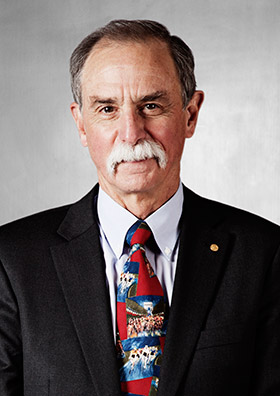
\includegraphics[width=.2\textwidth]{wineland.jpg}
  \caption{David Wineland in 2012.\\ Source: \textit{nobelprize.org}}
\end{wrapfigure}
David Wineland was born the same year as Serge Haroche on February 24, 1944,
in Wauwatosa, Wisconsin. His family moved to Sacramento, California in 1947
where he grew up and went to college. He describes his parents as marked by the
great depression emphasizing ``the importance of frugality and getting a good
education''~\cite{dwbio}. Having finished highschool in 1961, Wineland enrolled
for a Math Major at the University of California. He soon realized that, working
hard enough, he could make it too the top of his class. Still in his Junior year
he changed his university and subject and took up a Physics Major at Berkeley.
At the end of his undergraduate studies in physics he was not sure were to apply
for a Master and PhD, but asking his classical mechanics teacher helped a lot:
``he recommended Harvard, so I applied there''. This said he started his studies
at Harvard University in 1965 and soon joined the group of Norman Ramsey.\footnote{Nobel
prize in physics 1989 ``for the invention of the separated oscillatory fields
method and its use in the hydrogen maser''}

\subsection{Doppler Cooling}

\subsection{Trapping Single Ions}

\subsection{Ion Quantum Jumps}

\subsection{Sideband Cooling}

\subsection{Quantum Logic Gate}
